\section{Undertaken Research}\label{sec:research}

%Experiments:
%\begin{itemize}
    %\item Varying assimilation period and ensemble size, constant population
    %\item Varying assimilation period and population, constant ensemble size
    %\item Varying ensemble size and population, constant assimilation period
%\end{itemize}

%Visualisations:
%\begin{itemize}
    %\item Heat map of errors for ap vs es, ap vs pop, es vs pop
    %\item Snapshot of model with ensemble members linked to relevant states
%\end{itemize}

As outlined in Chapter \ref{sec:method}, the Ensemble Kalman Filter is a data
assimilation method which aims to approximate the effect of the original Kalman
Filter by representing the state of the model on which it is operating as an
ensemble of state samples.
The aim of applying this ensemble method is to overcome the difficulties
encountered by the original Kalman Filter when being applied to non-linear
models, and when attempting to propagate the state covariance matrix for models
with high dimensionality.
This method has been applied to an agent based model of pedestrian movement
(documented in Section \ref{sub:research:model}) with a view to reducing the error
in the model with respect to the ground truth.
It should be noted that this section adopts the common terminology of
``forecast'' to mean the state predicted by the model before updating, and
``analysis'' to mean the state after updating.

This section will present the results of the initial experiments that have been
undertaken.
These experiments seek to show that the Ensemble Kalman Filter is effective in
reducing simulation error when implemented for a simple agent-based model, and
furthermore seeks to explore the impact of different factors on this error
reduction.
This will be achieved by first showing the impact of the filtering process on
the model state, in particular focussing on a single agent in the model.
It will then be showed how the simulation error varies over time, comparing the
evolution of the error in the forecast, the error in the analysis and the error
in the observations.
Finally, results will be presented for the exploration of the impact of varying
ensemble size, assimilation period, population size and measurement error on the
effectiveness of the filter.

\subsection{Model}\label{sub:research:model}

The Ensemble Kalman Filter outlined in Section \ref{sub:method:enkf} is
implemented in conjunction with a pedestrian agent-based model known as
\texttt{StationSim}\footnote{https://github.com/Urban-Analytics/dust/blob/master/Projects/ABM\_DA/stationsim/stationsim\_model.py}
which aims to simulate pedestrians crossing from one side of the station to the
other.
StationSim has been developed under an object-oriented framework, and as such
both the model and the agent are represented by classes.
The state of each agent, $a_i$, comprises of its positions in two-dimensional continuous space:
\begin{equation}
    a_i = \left( x_i , y_i \right).
\end{equation}
The state of the model, $m$, comprises of the collection of all of the agents in the
model:
\begin{align}
    m &= \left[ a_0 , \ldots , a_N \right]^T \nonumber \\
      &= \left[ x_0 , y_0 , \ldots , x_N , y_N \right]^T,
\end{align}
where $N$ is the population size.
At each time-step, the model state is evolved by sequentially evolving the
agents.

The model is initialised by passing a number of arguments to the constructor,
including the number of agents in the population and the dimensions of the
rectangular environment.
Upon initialisation, the model generates a population of agents, each of which
are randomly allocated the following:
\begin{itemize}
    \item Entrance through which to enter the environment.
    \item Exit through which to leave the environment.
    \item Speed at which to traverse the environment.
\end{itemize}
As shown in Figure \ref{fig:sample_model_run}, entrances are located on the
left-hand side of the rectangular environment, and exits are located on the
right-hand side of the environment, with each agent seeking to traverse the
environment from their respective entrance to their respective exit.
Agents' motion across the environment is largely linear until they interact with
each other.
Where the paths of agents intersect in time and space, crowding occurs.
Faster agents attempt to pass slower agents, at times getting stuck behind them
--- this can be observed in the trails show in Figure \ref{fig:sample_model_run}
at $(x, y) \approx (65, 55)$.

The above phenomenon is a consequence of the agent behaviour outlined in Figure
\ref{fig:step}.
In Figure \ref{fig:step} (and subsequently Figure \ref{fig:act_deact}), the
\texttt{status} variable refers to whether an agent is active or not; a
\texttt{status} of 0 indicates that the agent is not active but is waiting to
become active, a \texttt{status} of 1 indicates that the agent is active and is
traversing the system, a \texttt{status} of 2 indicates that the agent has left
the system and is no longer active.
This variable controls agents' activation and deactivation behaviours outlined
in Figure \ref{fig:act_deact}.
The crowding phenomenon occurs due to the behaviour described in Figure
\ref{fig:move}, whereby agents attempt to move as far directly towards their
target destination as possible.
If they are unable to proceed forward, they engage the \texttt{wiggle} behaviour
where by they choose to move up or down (in the $y$-direction) in an attempt to
pass the obstruction in front of them; the decision to move either up or down is
made randomly with each choice carrying an equal probability.

\subsection{Experimental Setup}\label{sub:research:experiments}

With the above model in mind, a set of experiments were designed.
This first involved confirming that the Ensemble Kalman Filter was effective in
reducing the simulation error.
We then went on to explore the way in which different factors impact the
performance of the Ensemble Kalman Filter when applied to an agent-based model.
In particular, the factors that were explored were:
\begin{itemize}
    \item \textbf{Ensemble Size}: The number of copies of the model that the
        filter maintains.
    \item \textbf{Assimilation Period}: The number of time steps between each
        successive observation being used to update the model states.
    \item \textbf{Measurement Error}: The standard deviation of the noise
        applied to the ground truth data in order to obtain observations.
    \item \textbf{Population Size}: The number of agents created in the model.
\end{itemize}

In order to undertake this investigation, a class was developed in Python to
represent the Ensemble Kalman Filter.
The Python class representing the model is passed to the filter class as an
argument, along with the filter ensemble size, the frequency with which the
filter should assimilate data, and parameters governing the observational noise.
Upon construction, an instance of the filter class creates an instance of the
model, referred to as the \texttt{base\_model}, which takes the parameters given
in Table \ref{tab:model_params}.
Subsequently, an ensemble of models is created by taking deep-copies of the
\texttt{base\_model}, thus ensuring that each of the ensemble members starts
with model- and agent-attributes that match those in the \texttt{base\_model}.

The instance of the filter class steps forward through time according to the
predict-update cycle.
At each predict step, each of the ensemble member models are stepped forward
once, along with the base model; the frequency with which the filter undertakes
the update step is governed by a parameter known as the
\texttt{assimilation\_period}.
Upon reaching the update step of each cycle, the state of each of the ensemble
member models is updated according to equations found in Section
\ref{sub:method:enkf}.
The ground truth for these experiments is taken to be synthetic data generated
by the \texttt{base\_model}; observations are then generated by adding normally
distributed random noise to the ground truth at each assimilation step.
Errors are calculated as the root-mean-squared error averaging over the
population of agents:
\begin{equation*}
    RMSE = \sqrt{\frac{1}{N} \sum_{i=0}^{N}
    \left( \hat{x}_i - x_i \right) ^{2}},
\end{equation*}
where $\hat{x}_i$ is the model state of the $i$th agent, $x_i$ is the ground
truth state of the $i$th agent and $N$ is the population size.

\paragraph{Experiment 1: Confirming that Ensemble Kalman Filter is effective}

This experiment aims to examine the impact of the Ensemble Kalman Filter on the
model state through the visual examination of the model state before and after
the update process.
This is achieved by running the Ensemble Kalman Filter implementation with the
filter and model parameters found in Tables \ref{tab:filter_params_12} and
\ref{tab:model_params_12} respectively.
The mean model state will be plotted for one of the agents in the model, along
with each of the positions for the agent in each of the ensemble of models and
the observed position, both before the update and after the update.
The expectation is that the update process reduces the uncertainty in the
model's estimate of the agent's position, and that the posterior estimate is
more accurate than the prior estimate.

\paragraph{Experiment 2: Exploring evolution of errors over time}

This experiments aim to compare the forecast error, the analysis error
and the observation error of the system, and examine how they each vary over
time.
In order to achieve this, 10 realisations of the system are run using the same
filter and model parameters found in Tables \ref{tab:filter_params_12} and
\ref{tab:model_params_12}.
The forecast, analysis and observation errors are extracted from each of these
realisations at each point in model time when the Ensemble Kalman Filter updates
the states of each of the models in the ensemble (i.e.\ every 50 time-steps).
The each set of errors are averaged over the realisations with a view to finding
the average behaviour for each and comparing how they vary over model time.

\paragraph{Experiment 3: Exploring the impact of filter parameters}

The third and final experiment seeks to explore the impact of variations in
filter parameters on filter performance --- in particular the impact of
assimilation period, ensemble size and measurement error (as outlined above).
This is achieved by running the system for a variety of parameter values shown
in Table \ref{tab:filter_params}, and analysing how the behaviour of the system
changes with an increasing population size.
For each combination of parameters, the system is run 10 times, each time
extracting the forecast, analysis and observation errors for each point in model
time at which the system is updated with observation data.
Outputs are averaged over both the realisations and the simulation time to
produce a individual forecast, analysis and observation error values for each of
the parameter combinations.
These are plotted as heatmaps, focusing on the variation in analysis error with
population size and the filter parameter of choice.
As the population size increases, the number of interactions between agents
increases, leading to more random decisions being made as a consequence of the
\texttt{wiggle} behaviour.
As a result, the predicted model states are likely to deviate further from the
ground truth.
It is expected that increasing the filter ensemble size will reduce this impact,
as should reducing the assimilation period.

\subsection{Results}\label{sub:research:results}

\paragraph{Experiment 1: Confirming that Ensemble Kalman Filter is effective}

Figure \ref{fig:250_single} shows the impact of the applying the Ensemble Kalman
Filter on one of the agents in the model.
The observation error is considered as the distance between the observed agent
state and the true agent state --- this remains unchanged between Figures
\ref{fig:before_250_single} and \ref{fig:after_250_single}; the forecast error
is the distance between the ensemble mean agent state and the ground truth agent
state in Figure \ref{fig:before_250_single}; the analysis error is the distance
between the ensemble mean agent state and the ground truth agent state in Figure
\ref{fig:after_250_single}.

It can be seen by in Figure \ref{fig:before_250_single} that the forecast error
is greater than the observation error.
Furthermore, it can be seen that the variance in the forecast error for the
ensemble members is large with some members lying as close to the ground truth
as the observed agent state and others lying approximately fours times as far
away.
The majority of the variation occurs in the $x$-direction, indicating that in
the case of some ensemble member models the agent in question likely became
involved in some crowding and became stuck behind other agents, whilst in other
ensemble member models the agent may be ahead of the crowd and has proceeded
unimpeded.

Comparing Figures \ref{fig:before_250_single} and \ref{fig:after_250_single}
reveals two points.
The first is that ensemble mean agent state lies much closer to the ground truth
agent state --- closer than the observed agent state.
Indeed, the improvement in accuracy is such that the ensemble mean agent state
at almost exactly the same location as the ground truth agent state.
Beyond this, it can be seen that the variance in the error for the ensemble
members has greatly reduced.
These two observations suggest that the Ensemble Kalman Filter is effective in
improving the accuracy with which the model can simulate the system.

To ensure that this result is not restricted to the individual agent, the next
experiment will go on to average the errors over the whole agent population.

\paragraph{Experiment 2: Exploring evolution of errors over time}

This experiment seeks to consider the variations in error over time.
In particular Figure \ref{fig:error_evolution} consists of three sub-plot, in
each case showing the evolution of average error per agent over time.
The experiment is run for 10 realisations, each time using the same model and
filter parameters.
Each dashed line in Figure \ref{fig:error_evolution} is indicative of a single
realisation, whilst the solid line is the average over all realisations.


\paragraph{Experiment 3: Exploring the impact of filter parameters}

Figure \ref{fig:es_heatmap}, \ref{fig:ap_heatmap}, \ref{fig:std_heatmap}

\subsection{Conclusion}\label{sub:research:conclusion}

This is ok, but we've got some issues

\newpage
\begin{table}[h]
    \centering
    \begin{tabular}{@{}ll@{}}
        \toprule
        Variable                       & Value                         \\ \midrule
        Number of iterations           & 300                           \\
        Assimilation period            & 50                            \\
        Ensemble size                  & 10                            \\
        Observation standard deviation & 1.0                           \\ \bottomrule
    \end{tabular}
    \caption{Table of filter parameters for experiments
    1 and 2.}\label{tab:filter_params_12}
\end{table}

\begin{table}[h]
    \centering
    \begin{tabular}{@{}ll@{}}
    \toprule
        Variable            & Value                 \\ \midrule
        Population size     & 20                    \\
        Number of entrances & 3                     \\
        Number of exits     & 2                     \\
        Environment height  & 100                   \\
        Environment width   & 200                   \\ \bottomrule
    \end{tabular}
    \caption{Table of model parameters for experiments
    1 and 2.}\label{tab:model_params_12}
\end{table}

\begin{table}[h]
    \centering
    \begin{tabular}{@{}ll@{}}
        \toprule
        Variable                       & Value                         \\ \midrule
        Number of iterations           & 300                           \\
        Assimilation period            & $[2, 5, 10, 20, 50]$          \\
        Ensemble size                  & $[2, 5, 10, 20, 50]$          \\
        Observation standard deviation & $[0.5, 1.0, 1.5, 2.0, 2.5]$   \\ \bottomrule
    \end{tabular}
    \caption{Table of filter parameters for experiments.}\label{tab:filter_params}
\end{table}

\begin{table}[h]
    \centering
    \begin{tabular}{@{}ll@{}}
    \toprule
        Variable            & Value                 \\ \midrule
        Population size     & $[5, 10, 15, 20, 25$] \\
        Number of entrances & 3                     \\
        Number of exits     & 2                     \\
        Environment height  & 100                   \\
        Environment width   & 200                   \\ \bottomrule
    \end{tabular}
    \caption{Table of model parameters for experiment.}\label{tab:model_params}
\end{table}

%\begin{figure}[h]
    %\centering
    %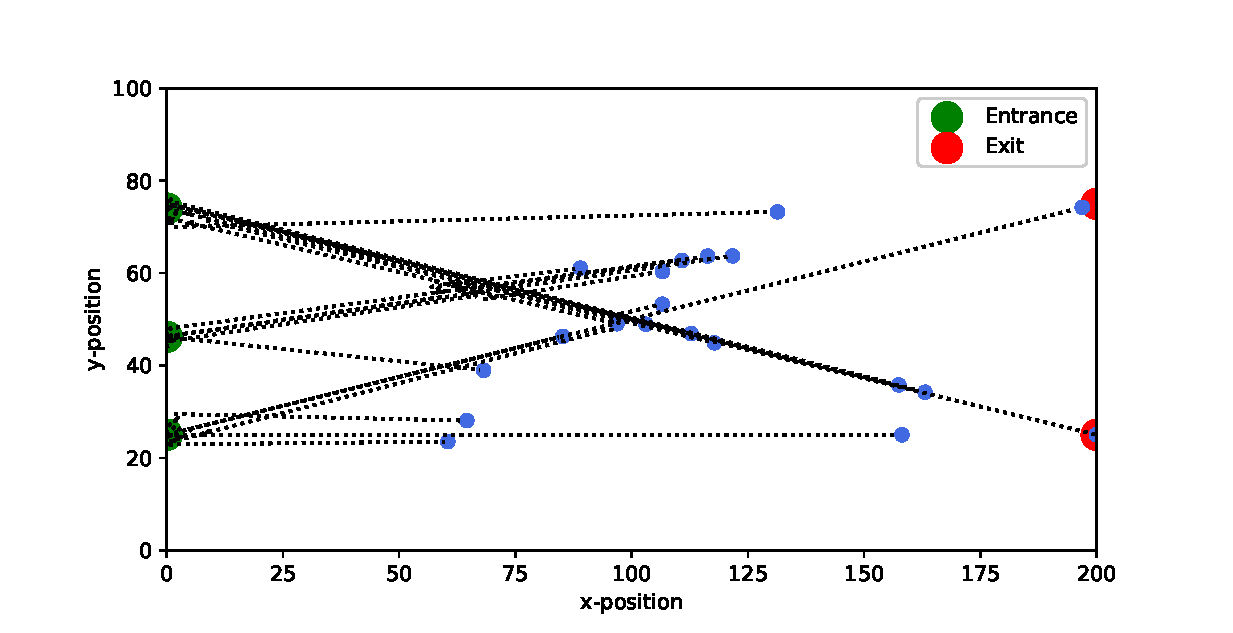
\includegraphics[width=\textwidth]{sample_model_run.eps}
    %\caption{Example run of StationSim for 20 agents; agents enter environment
    %through entrances on left and leave through exits on right.}
    %\label{fig:sample_model_run}
%\end{figure}

\begin{figure}[!htb]
    \centering
    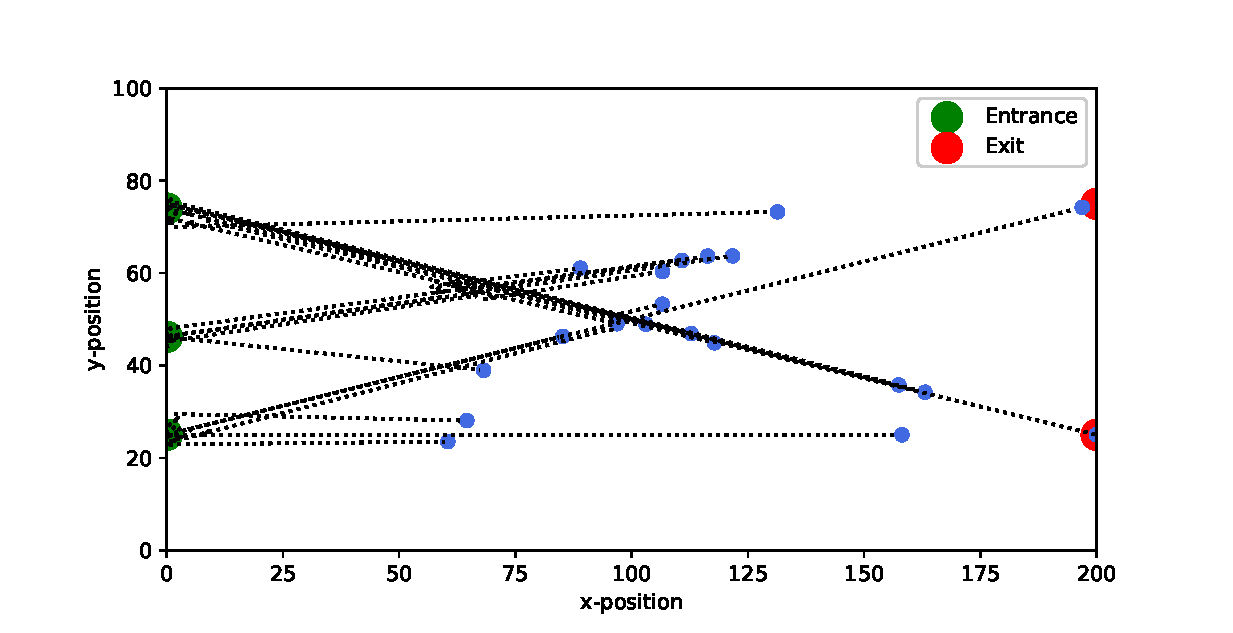
\includegraphics[width=0.8\textwidth]{sample_model_run.eps}
    \caption{Sample model run.}\label{fig:sample_model_run}
\end{figure}

\begin{figure}[!htb]
    \centering
    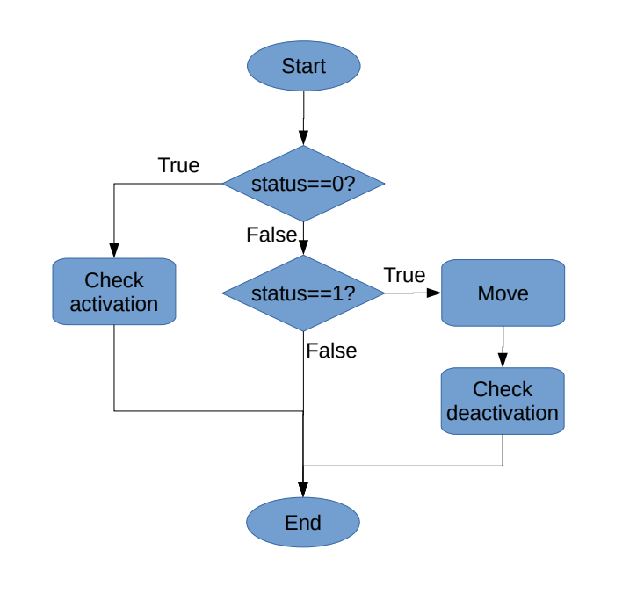
\includegraphics[width=0.8\textwidth]{step.eps}
    \caption{Flow diagram of agent step behaviour. Activation and deactivation
        behaviours are defined in Figure \ref{fig:act_deact}; movement behaviour
    is defined in Figure \ref{fig:move}.}\label{fig:step}
\end{figure}

\begin{figure}[!htb]
    \centering
    \begin{subfigure}[h]{0.4\textwidth}
        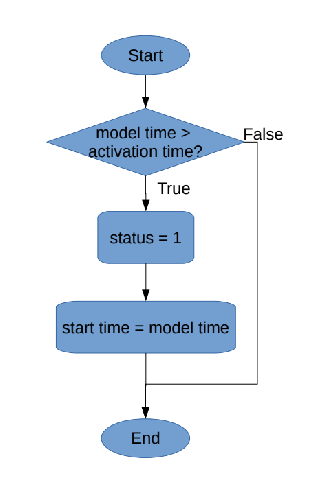
\includegraphics[width=\textwidth]{activate.eps}
        \caption{Activation}\label{fig:act_deact:act}
    \end{subfigure}
    ~
    \begin{subfigure}[h]{0.3\textwidth}
        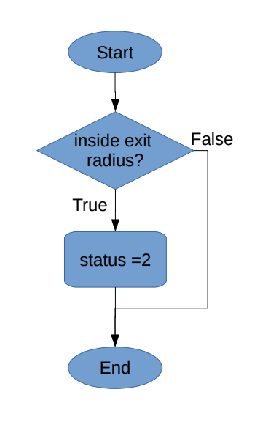
\includegraphics[width=\textwidth]{deactivate.eps}
        \caption{Deactivation}\label{fig:act_deact:deact}
    \end{subfigure}
    \caption{Flow diagrams of agent behaviours for activation and deactivation.}
    \label{fig:act_deact}
\end{figure}

%\begin{figure}[h]
    %\centering
    %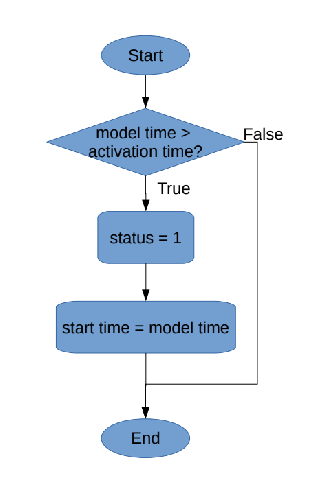
\includegraphics[width=0.5\textwidth]{activate.eps}
    %\caption{Flow diagram of agent step behaviour}
%\end{figure}

%\begin{figure}[h]
    %\centering
    %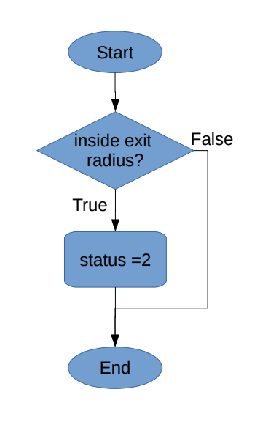
\includegraphics[width=0.5\textwidth]{deactivate.eps}
    %\caption{Flow diagram of agent step behaviour}
%\end{figure}

\begin{figure}[!htb]
    \centering
    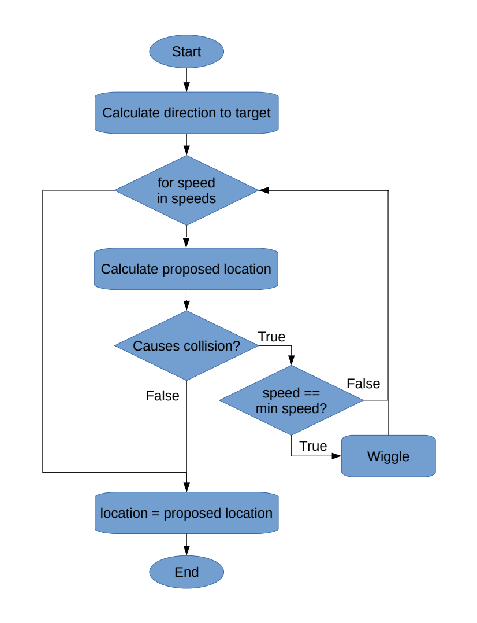
\includegraphics[width=0.8\textwidth]{move.eps}
    \caption{Flow diagram of agent movement behaviour.}\label{fig:move}
\end{figure}

\begin{figure}[!htb]
    \centering
    \begin{subfigure}[h]{\textwidth}
        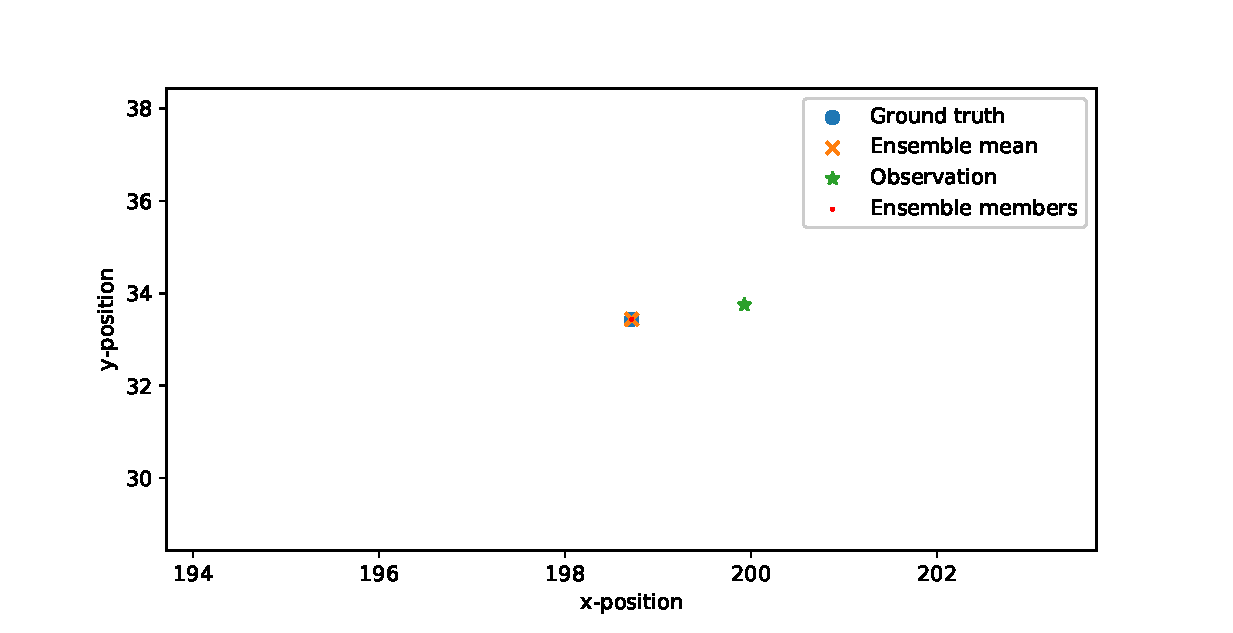
\includegraphics[width=\textwidth]{before_update_250_single.eps}
        \caption{Before}\label{fig:before_250_single}
    \end{subfigure}

    \begin{subfigure}[h]{\textwidth}
        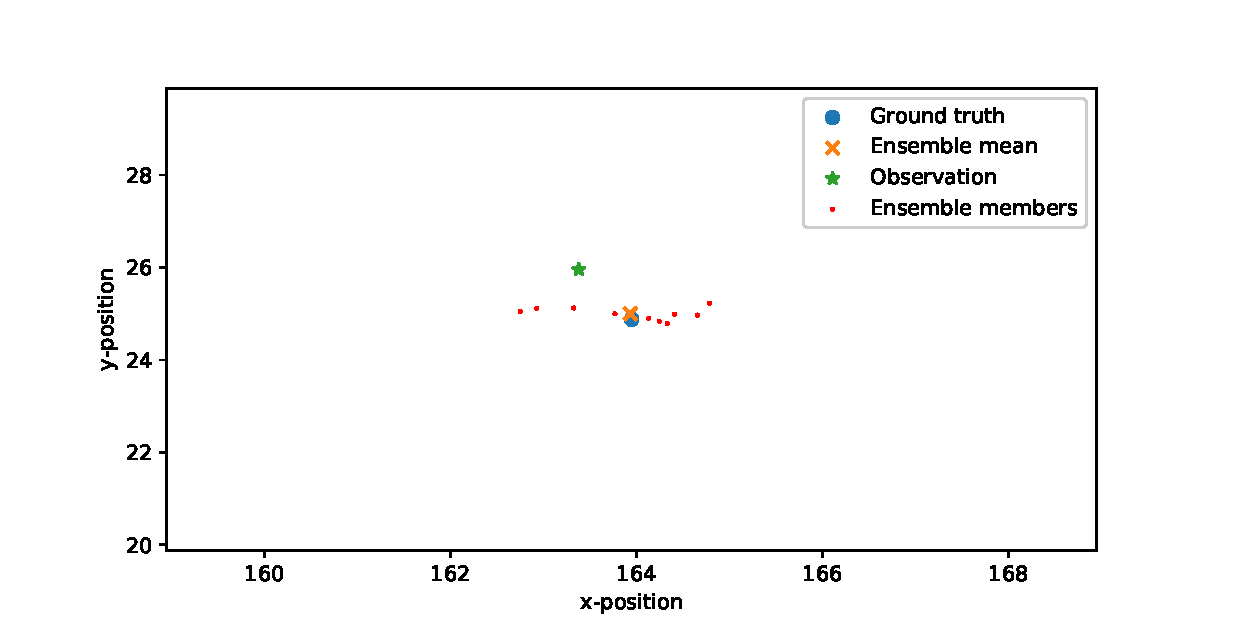
\includegraphics[width=\textwidth]{after_update_250_single.eps}
        \caption{After}\label{fig:after_250_single}
    \end{subfigure}
    \caption{Comparison of model state before and after updating via the
    Ensemble Kalman Filter, focusing on a single agent in the system.}
    \label{fig:250_single}
\end{figure}

\begin{figure}[!htb]
    \centering
    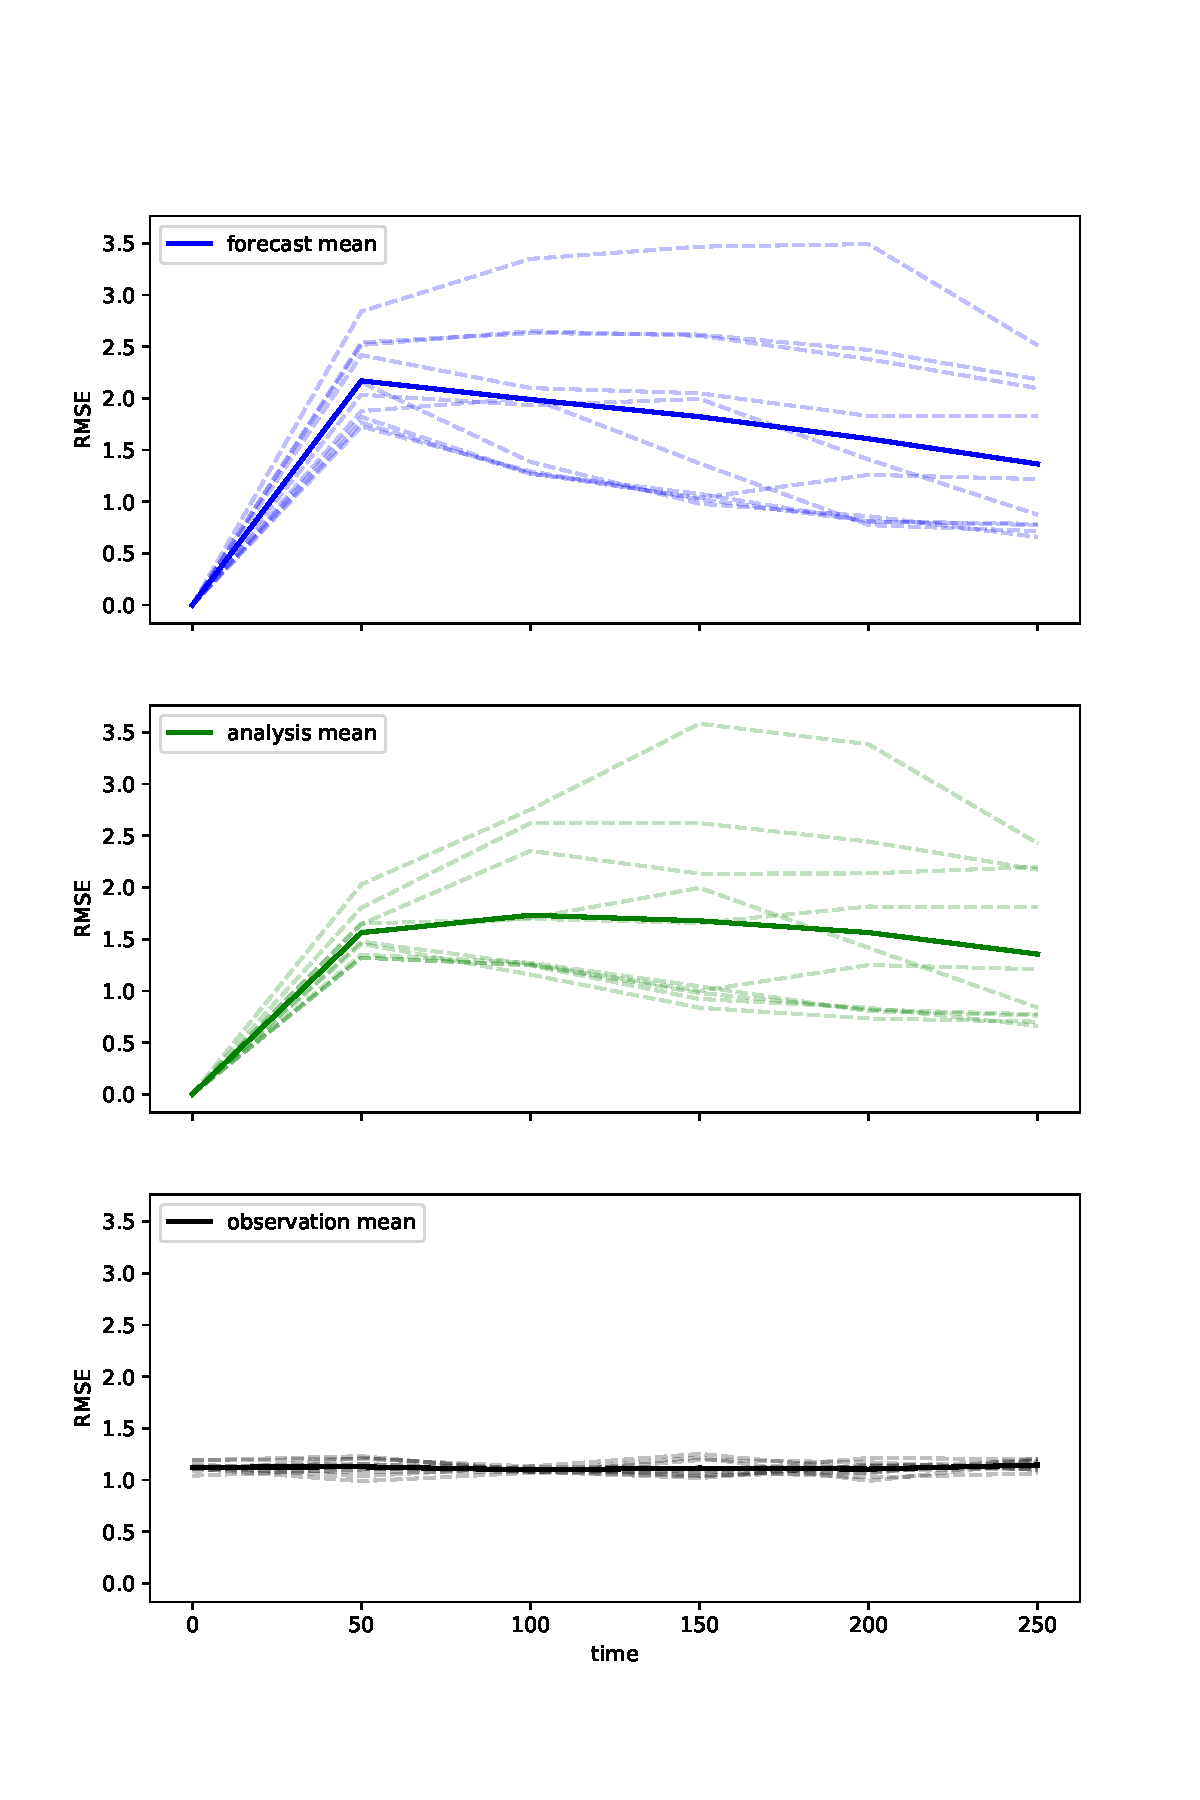
\includegraphics[width=\textwidth]{all_results.pdf}
    \caption{Evolution of forecast error, analysis error and observation error
    over model time; solid lines indicate mean, dashed lines indicate individual
realisations.}\label{fig:error_evolution}
\end{figure}

\begin{figure}[!htb]
    \centering
    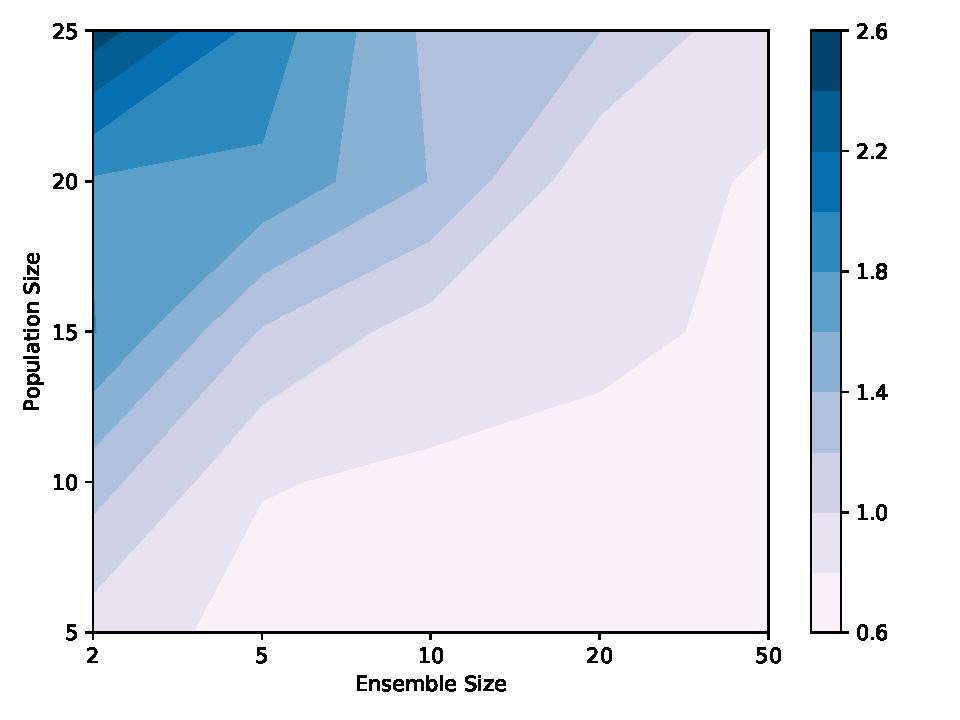
\includegraphics[width=0.8\textwidth]{ensemble_size_population_size.pdf}
    \caption{ES heatmapt}\label{fig:es_heatmap}
\end{figure}

\begin{figure}[!htb]
    \centering
    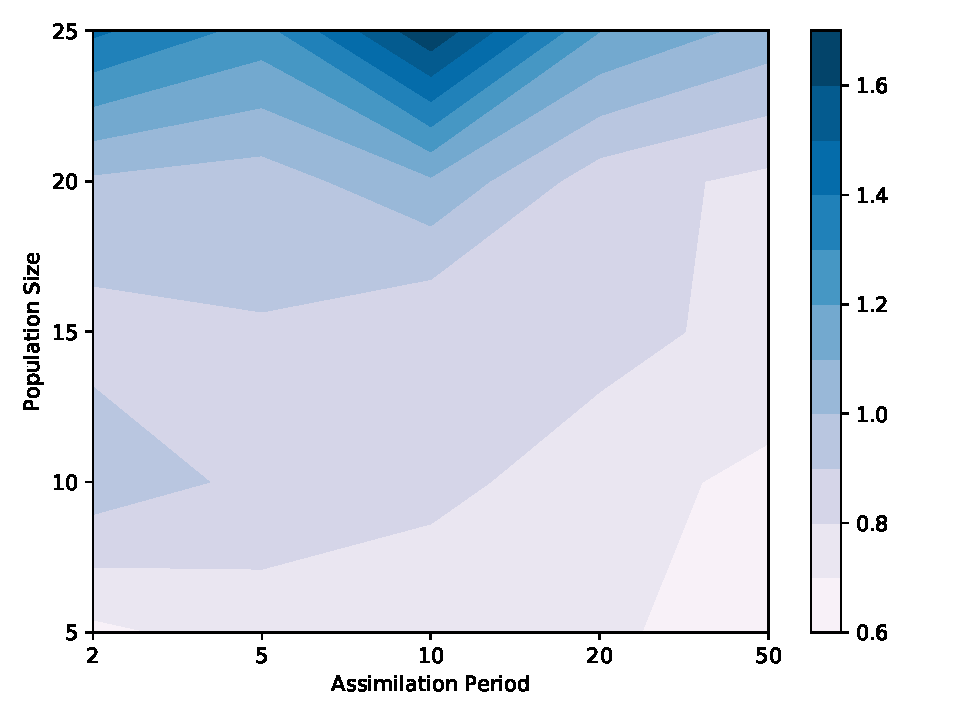
\includegraphics[width=0.8\textwidth]{assimilation_period_population_size.pdf}
    \caption{AP heatmap}\label{fig:ap_heatmap}
\end{figure}

\begin{figure}[!htb]
    \centering
    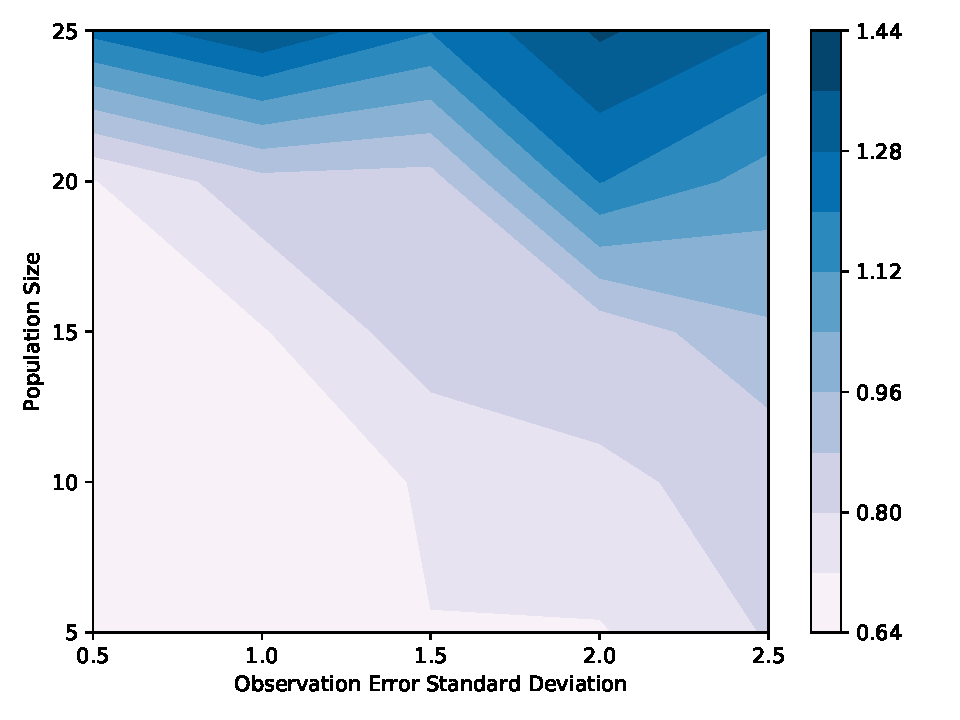
\includegraphics[width=0.8\textwidth]{std_population_size.pdf}
    \caption{STD heatmap}\label{fig:std_heatmap}
\end{figure}

